\documentclass{article}


\usepackage{authblk}
\usepackage{listings, chngcntr}
\usepackage{textcomp}
\usepackage{float}
\usepackage[T1]{fontenc}
\usepackage{indentfirst}
\usepackage{graphicx}
\usepackage{array}
\usepackage{caption} 
\usepackage{hyperref}
\usepackage{verbatim}
\usepackage{float}
\usepackage{subcaption}
\usepackage{gensymb}
\usepackage{amsmath}
\usepackage{geometry}
\usepackage{multirow}
\usepackage{listings}


\geometry{
    a4paper,
    left=30mm,
    right=30mm,
    top=30mm,
    bottom=40mm
}

\begin{document}

\title{Single Photon Interference}
\author[1]{Woojin Han}
\affil[1]{Seoul National University, Seoul 151-747, Korea}
\maketitle

\begin{abstract}
  In this experiment, I suggested the statistical criteria, dependent parameters and dimensionless parameters and applied them to the interference patterns.
  The laser and weak bulb are used for the pattern, proving that the intensity of light does not affect the significant parameters.
  Also, the published specification of the slit is verified by the 6 different experiments.
  The fitting method for sensible parameters is suggested.
  The method is proved and applied to consider the wavelength dispersion of the light source, which may not be easily gathered from convolution-fitting results.
  The wave packet size and the number counts of the photon are calculated and check the single photon limit condition.
  Finally, the Python module for fitting, plotting, partial fitting, and convenient data manipulation is made and uploaded.
  The fully working files and the raw data are also uploaded, the successor may download the module and use it.
\end{abstract}

\section{Introduction}
 The experiment of light interference is very significant in research of early quantum mechanics.
The interference pattern is used to explain the wave-like nature of light, which is rejected by the photon model.
In this experiment, we checked the light interference pattern in the weak amplitude limits of light, to find the quantum duality of light.
But, the signal is too small and wide variance the statistical method must be checked.
In \ref{intro: data analysis} section, I uploaded to the public the analysis module and the fully activating code.
Secondly, the data points are tightly measured for high trust in the results.

The laser interference experiment is performed in double and single slits for each slit and is statistically verified.
The wavelength dispersion value in dimensionless form is suggested, and its fragile limitation is checked.
Also, the wavelength dispersion value in clever fitting is applied and successfully matches the published specification value of the experimental tool.
The validity check and the partial fitting method are used to prove the single-photon limit experiment results can be explained by the math used in multi-photon limits.


\subsection{Fitting Functions: Statistical Verification}
\label{intro: statistical_setup_fitting_method}
 The results take the form of two different experimental values, the detector voltage in the laser experiment, and the pulse count data in the single photon limit experiment.
 Firstly, the laser experiment analysis method is described.
 The slit has three different significant values to affect the interference pattern.
 As Fig. \ref{fig: slit_specs}, $\sigma_{1,2}$, the slit width of right, and left in sight of align each respectively. $\Delta$, the distance between two slits.
 For convenient naming to fitting variables, I name the slit specification parameters in the Greek alphabet.
 \begin{figure}[H]
    \centering
    \begin{subfigure}[b]{7cm}
        \centering
        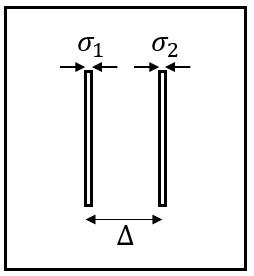
\includegraphics[width=3cm]{../results/slit_specs.png}
        \caption{}
    \end{subfigure}
    \hfill
    \caption{Schematic model of the slit}
    \label{fig: slit_specs}
\end{figure}
 By simple calculations, the double slit results which assume $\sigma1 = \sigma2 = \sigma$ and no spectral dispersion, in each the wavelength of the laser is uniform enough to $\lambda$, follows equation \ref{equation: raw double slit}.
 The fitting parameters are $c, I, d_1, d_2$ which are the center of the detector slit, the center intensity, and the spatial parameters of slit width and distance each.
 Since the values of $\sigma$ and $L$ have an ambiguity of absolute value, only their ratio matters.
 Therefore, I select $d_1, d_2$ instead.


 \begin{align}
     I(x;c,I,d_1,d_2) = &I \left( \frac{\sin(\pi \frac{x-c}{d_1})}{\pi \frac{x-c}{d_1}} \right)^2 (\cos(\pi \frac{x-c}{d_2}))^2  \nonumber \\
     &d_1 = \frac{L \lambda}{\sigma}, \quad d_2 = \frac{L \lambda}{\Delta}  \label{equation: raw double slit}
 \end{align}

 For modeling the dispersed nature of the laser wavelength, the Lorentzian distribution is used.
 Since the laser emits light in band gap resonance, the assumption is valid.
 Equation \ref{equation: double slit light dispersion} shows the Lorentzian profile of the wavelength.
 $\gamma$ is the FWHM value of the wavelength, $\Gamma$ is dimensionless factor of the distribution.
 To detour the ambiguity of $\lambda$ and $\gamma$, I used $\Gamma$ as a fitting parameter.
 $d_i$, the fitting parameters are linear to $\lambda$, the probability density of $d$ while $d_i$ is the central value can be calculated as follows.

 \begin{align}
    &g(\lambda; \gamma) = \frac{1}{\pi} \frac{\frac{\gamma}{2}}{\lambda^2 + (\frac{\gamma}{2})^2} \nonumber \\
    &\gamma = \lambda \times \Gamma \nonumber \\
    &P(d|d_i) = g(\frac{d-d_i}{d_i};\Gamma) \label{equation: double slit light dispersion}
 \end{align}
 
 Finally, the fitting equation is \ref{equation: modified double slit}.
 This type of fitting is written as Laser Broadening Fitting(LBF).
 The integrand function is the simple double-slit function in \ref{equation: raw double slit}.

 \begin{equation}
    I(x;c,I,d_1,d_2,\Gamma) = \int I(x;c,I,d_1(1+\alpha),d_2(1+\alpha),\gamma) g(\alpha;\Gamma) d\alpha
    \label{equation: modified double slit}
 \end{equation}

 In the asymmetric setting in each case of $\sigma_1 \neq \sigma_2$ changes the single slit interference part either.
 But, the condition leads to overfitting since there are too many parameters compared to the data points.
 Therefore, I assume $\sigma_1 \sim \sigma_2$ which gives the difference in the amplitude of light.
 This type of fitting is written as Asymmetric Correction Fitting(ACF).

 \begin{equation}
    I(x;c,I,d_1,d_2, I_2) = \left( \frac{\sin(\pi \frac{x-c}{d_1})}{\pi \frac{x-c}{d_1}} \right)^2 \frac{1}{4}(I + I_2 + 2 \sqrt{I I_2}\cos(2\pi \frac{x-c}{d_2})) 
 \end{equation}
 
 In the laser experiment, many photon limits results are fully explained by those functions.
 But, in the bulb experiment, single photon limit results have different types of measurement occurring.
 The Photomultiplier Tube (PMT) detector amplifies the small size input to the large signal.
 And, the measurement data is the count of the pulse which has the amplified signal over a certain threshold.
 The amplification is controlled by the factor of PMT, High Voltage (HV).
 I assume two things to make a model of PMT pulse count data.
 First, the photon detection probability is uniform of the timescale $1s$.
 Secondly, each photon gives excitation to PMT in uniform amplitude.
 Let single-photon excites the PMT in the amplitude of $V_0$ for $\tau$ seconds.
 And, $n$ number of photons emits in unit time $t_0 >> \tau$ by assumption.
 Then, the probability of the signal $V$, $P(V;j)$ has a relation of equation \ref{equation: PMT}.
 Each photon has the probability to excite the PMT in a certain time for $2\tau/t_0$.
 So, the number of photons follows binomial distribution $B(n,2\tau/t_0)$.
 \begin{equation}
    P(V>(threshold);j) \sim A e^{-2\tau j}
    \label{equation: PMT}
 \end{equation}

 In the definition of $j = n/t_0$, the probability of a pulse count is exponentially related to the input signal.
 By the signal resolution time, the Pulse Counter/Interval Timer(PCIT) value is exponentially dependent on the input signal.
 Moreover, by the assumption of the binomial distribution, the variance of the PCIT value is proportionally linear to the mean value.
 In the fitting of single photon limits, I may check the $1\sigma$ boundary of multiple experiment results, to check the reliability of the fitting method.


 The nonvanishing problem may also be explained by the rejection of the Fraunhofer approximation.
 Those two slit intensities may differ for the distance between two optical routes.
 But this opinion is simply neglected by the precision of this experiment.
 The route distance difference is about $(\frac{\Delta}{L})^2 \sim (\frac{10\mu m}{10 cm})^2 = 10^{-8}$.
 This means that the difference between the route may affect the intensity results, but the effect is negligible with the natural error of $10^{-4}$, voltage measurement.
 Also, the slit size difference $\sigma_1 \neq \sigma_2$ regime is dominating the Fraunhofer correction.
 So, if the fitting function which considers the optical length difference fits well, the fitting data must not be trusted by this p-value test.

 Just like the previous example, the function fits well with many variables.
 Also, there are a lot of parameters in each fitting function, the fitting results may fall into local minima and lose their physical meaning.
 To avoid overfitting, I double-checked the parameters in each fitting method.
 The parameter $c, I,d_i$ must have similar values since they have the physical backgrounds of slit specification.
 If the parameters are significantly different of $2 \sigma$, a p-value of 0.05, I avoid using the fitted results.
 To help the statistical verification, a specially built module is informed at \ref{intro: data analysis}.


 \subsection{Data Analysis Module}
\label{intro: data analysis}
 To fit various functions, the codes are too messy in dealing with data sets.
 Also, the fitting parameters are too many to optimize in strange local minima lots of times.
 The modulation of the initial parameters is not good enough to try in many data sets.
 Therefore, I made the module of fitting and plotting.
 The idea is that the fitting parameters have a relation with the roughly fitted parameters.
 For example, $[c, I,d_1,d_2]$ results in equation \ref{equation: raw double slit} fitting are similar to the results of $[c, I,d_1,d_2,\Gamma]$ in equation \ref{equation: modified double slit}.
 If is not, the physical meaning of each parameter is infringed, which means the results are overfitted.
 Therefore, I made an input of \verb|rough_fitting_functions| and \verb|fitting_param_query| which both take a role in roughly fitting the data itself, to avoid hard manipulation of initial parameters.

 \begin{lstlisting}[language = Python]
    laser_modified_fig = spi.phys_plot(
            data_set_list,
            lambda x: x.parameters,
            lambda x: x.results[0],
            {'align': 3, 'exp_type': 'double_slit'},
            fitting_function= modified_function,
            rough_fitting_functions = [rough_1,fitting_function],
            fitting_param_query = [None,lambda x: [*x[:4],1e-2]],
            p0_function = laser_double_slit_param_setting,
            truncate = lambda x: True if x<0.7 else False,
            export_param_statics = "export.txt"
        )  
 \end{lstlisting}

 For example, above is the example usage of \verb|spi.phys_plot| method.
 The first two inputs are the $x, y$ variables of the plot.
 So, the function will plot the \verb|x.results[0] - x.parameters|.
 I labeled the experiment as align trial 3, the experiment type is double slit.
 And the following \verb|modified_function| is the final fitting equation.
 The \verb|rough_1, fitting_function| are the roughly fitting functions like equation \ref{equation: raw double slit}.
 Sometimes the parameter numbers or the enumerate may change by the functions.
 For example, there are 4 parameters until \verb|fitting_function|, but we need 5 parameters in \verb|modified_function|.
 Then the fitting parameter should follow the query, in this case, \verb|lambda x: [*x[:4],1e-2]| which adds the fifth parameter as $10^{-2}$.
 Moreover, the method exports the parameters in the form of \LaTeX tabular environment in \verb|export_param_statics|.
 The exported example is like \ref{fig: tabular example}.

 \begin{figure}[H]
    \centering
    \begin{tabular}{c|c|c|c}
        \centering
        & & &  \\ \hline 
        1double slit 1& $0.234\pm 1.54e-08$& $0.042\pm 6.522e-06$& 0.9920
    \end{tabular}
    \caption{example output of phys plot method}
    \label{fig: tabular example}
\end{figure}
By using this method, I can fit an enormous amount of data points without wasting time setting initial parameters, or writing the parameters down in the report.
Every code is uploaded in \cite{github}.

\section{Methods}
\label{methods: start}
Apparatus: PMT, PCIT, Oscilloscope, Slits (\cite{spi_spec}).
The slit spacing and its width are published as Fig. \ref{fig: slit_specs_data}.
The laser wavelength is $670 \pm 20 [nm]$, and the bulb interference filter transfers $546 \pm 10 [nm]$ wavelength light in the Lorentzian profile.
The U channel is the main passage of the light, transferring the single slit, double slit, blocker and detector slit in order.
The distance parameter $L, L_0, L_1$ is shown in Fig. \ref{fig: u_channel_specs}, the distance from the double slit to the detector, the distance between the single slit and the double slit, the width between the double slit and the blocker respectively.
$L = 49.81 [cm]$, $L_0 = 32.50 [cm]$, and $L_1 = 0.70 [cm]$ is the measured data of the U channel.

\begin{figure}[H]
    \centering
    \begin{tabular}{  |m{2cm} | m{2.5cm} | m{2.5cm} | m{2.5cm}|  } 
      \hline
      Slit No.& $\Delta [mm]$& $\sigma_1 [mm]$ & $\sigma_2 [mm]$ \\ 
      \hline
      \hline
        14 & $ 0.35 \pm 0.01$& $0.09 \pm 0.01$ & $0.09 \pm 0.01$\\
      \hline
        15 & $ 0.40 \pm 0.01 $& $0.09 \pm 0.01$ & $0.09 \pm 0.01$\\
      \hline
       16 &$ 0.45 \pm 0.01 $& $0.09 \pm 0.01$ & $0.09 \pm 0.01$\\
       \hline

    \end{tabular}
    \caption{Published slit specification data}
    \label{fig: slit_specs_data}
\end{figure}

\begin{figure}[H]
    \centering
    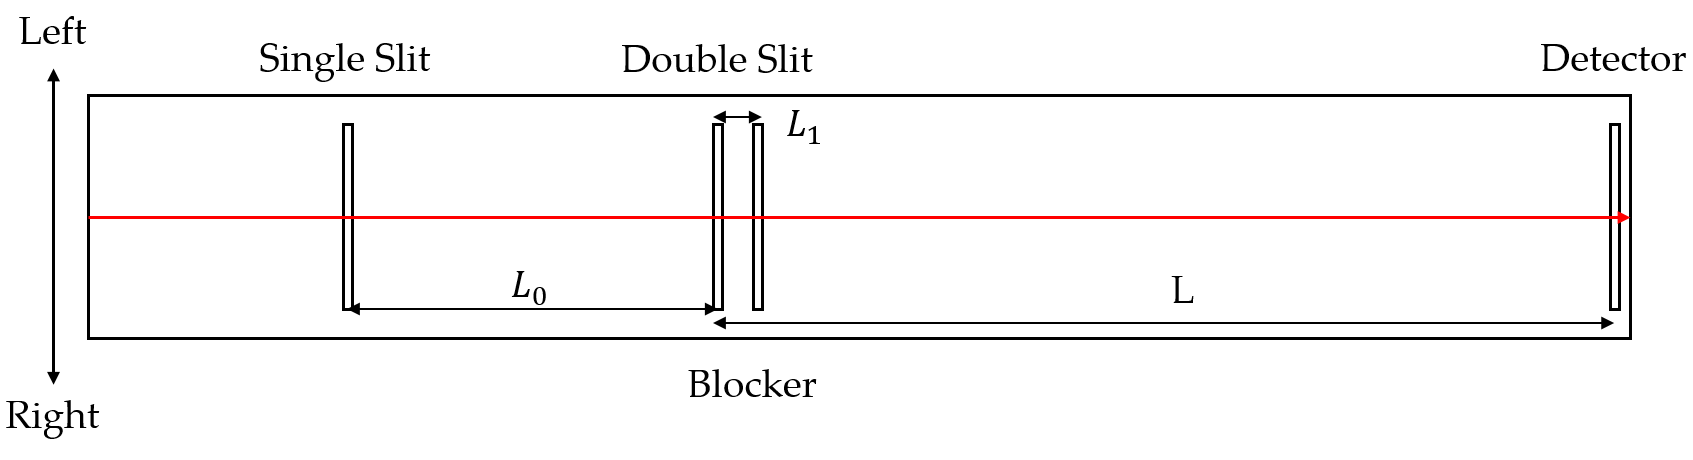
\includegraphics[width=13cm]{../results/u_channel_spec.png}
    \hfill
    \caption{
        Schematic model of U Channel, the laser alignment is represented in the red line, and each slit is plotted in a small box.
        The term left and right definition is also shown.
    }
    \label{fig: u_channel_specs}
\end{figure}
 
\subsection{Laser Experiment}
The multi-photon limit experiment uses the laser as a light source.
The align is fixed for the total measurement, but can not be regenerated.
Therefore, I label the experiment set as aligned number and experiment type.
For each alignment trial, the experiment has done in the double slit, right single slit, and left single slit using a blocker.
For example, in alignment number 1, the double-slit data and the single-slit data are measured.
A total of six alignments are done, in diverse slit conditions.
The data are measured in distance intervals of $0.0025 [cm]$, for $0 - 7 [cm]$. about 300 data points are measured for each experiment type.


\subsection{PMT Threshold}
The PMT has two parameters to control, High Voltage(HV) and the Threshold.
If the HV is too high, the PMT will amplify the dark noise signal into a visible photon signal, which must be avoided.
Besides, if the HV is too low, the PMT will not detect the photon signal and the module have a bad resolution.
The threshold parameter is just the same as negative PMT modulation.
Properly setting the threshold parameter to make PCIT variance low, and setting HV appropriate to the threshold is necessary.
The PMT HV lower boundary is measured in bright conditions.
If the PCIT measurement is not enough visible in the PMT even in the brightest setting, the HV value is not valid.
Also, the PMT HV upper boundary is measured in dark conditions.
If the PCIT measurement is too excited in the PMT even in dark moments, the HV value is not valid.
I have measured 7 times each in 25 different HV values for two different threshold parameter settings.
And the final setting $(HV) = 720 [V], (threshold) = 18.4 [mV]$ has been double-checked with oscilloscope data.

\subsection{Bulb Experiment: Single Photon Limit}
The single-photon limit experiment uses the bulb as a light source.
The alignment is also fixed for the total measurement.
I label the experiment as the aligned number and experiment type and bulb intensity.
For each alignment number, I varied the experiment type in the double, and single slits, and the bulb intensity to 5 from 3, in various slit numbers.
The data are measured 7 times in each position in distance intervals of $0.005 [cm]$, for $0 - 7 [cm]$, about 1500 data points are gathered in each experiment type and bulb intensity.


\section{Results and Discussion}
The total codes and raw data of each parameter are uploaded to GitHub.
(\cite{github}, \url{https://github.com/WoojinHan24/Single_Photon_Interference}).
To clarify the file name and its content in \verb|./results/|, the appendix is shown in Fig. \ref{fig: file_appendix}.
The Python code only to run is \verb|main.py|, which imports \verb|single_photon_interference| module, fully generating the results folder itself.
The visibility and blocker positions are not that necessary in the actual results and discussion.
Also, the 11 alignments have been done, the listing of those values in the report seems pointless, in file \verb|spi_raw_data.xlsx| each sheet has the alignment detail data.



\begin{figure}[H]
    \begin{tabular}{  m{5.2cm} | m{8.7cm} } 

      file name& details \\ 
      \hline
      \hline
        spi raw data.xlsx & The raw data of whole experiment\\
      \hline
        laser(x y) raw fig.png & ACF plots of alignment number x, experiment type y\\
      \hline
        laser x raw param statics.txt & ACF parameter results in experiment type x\\
      \hline
        laser(x y) modified fig.png & LBF plots of alignment number x, experiment type y\\
      \hline
        laser x param statics.txt & LBF parameter results in experiment type x\\
      \hline
        PMT upper boundary ($x$).png & PCIT in different HV, for threshold $x$\\
      \hline
        PMT upper boundary statics.txt & Fitting parameter of PMT upper boundary plot\\
      \hline
        PMT lower boundary ($x$,$y$).png & PCIT in different HV, for threshold $x$, bulb intensity $y$\\
      \hline
        PMT lower boundary statics.txt & Fitting parameter of PMT lower boundary plot\\
      \hline
        sensor slit position ($x$).png & PCIT-position plot in bulb intensity of $x$\\
      \hline
        sensor slit statics.txt & Fitting parameter of sensor slit position plot\\
      \hline
        bulb($x$ y) fig.png & PCIT LBF plots of Slit No. $x$, experiment type y\\
      \hline
        bulb x param static.txt & LBF parameter results in experiment type x \\

    \end{tabular}
    \caption{file appendix of \cite{github}}
    \label{fig: file_appendix}
\end{figure}

Each subsection is labeled just as same with subsection from \ref{methods: start} respectively.
\subsection{Laser Experiment}
In this subsection, three slits results are plotted and fitted respectively.
For each slit, two figures are posted.
The first figure is the voltage [mV] - detector position [cm] plots of three different experiment types, the double slit, and the single slits of each side. 
The second figure is the table containing parameter statics of previous plots respectively.
The row exp is the experiment type, all means the double slit case, and the R, L means the single slit of the right, left side.
$c, I,d_1,d_2,\Gamma$ is the position of the center of the screen, and the center intensity, the proper distances, and the dispersion coefficient respectively which are defined as equation \ref{equation: modified double slit}.

The pair results of Silt No. 14 are illustrated in Fig. \ref{fig: 14_laser_plot}, \ref{fig: 14_laser_parmeters}.
The difference of $c$ value between R, L results, $c_R - c_L$ is $\Delta$ in the theoretical model.
Because the $c_R, c_L$ is the position of the intersection point extension of each slit hole.
But, by backlash error, we can not find a relation between the different experiment types.
Also, note that the $\Gamma$ value is too fragile in its optimization.
Besides the parameters of $c, d_i$, the $\Gamma$ parameter changes its optimal value sensitively reacting to other parameters.
So, I only used $c, I,d_i$ values in single distribution fitting, and discuss the data of wavelength and dispersion ($\Gamma$) below with other slits results.
It is fine to check $c, I,d_i$, which is stable in its results in the variance of other parameters.
Except for $\Gamma$, by the statistical criteria I made, each parameter has a similar value with the other experiment in the same alignment, the LBF fitting is valid in Slit No. 14.
Especially $d_1$ is an important parameter that holds the information of slit width($\sigma$), is the same in $1\sigma$.
As mentioned at \ref{intro: statistical_setup_fitting_method}, $d_i$ have a distribution of Lorentzian by light dispersion signal to FWHM ratio as $\Gamma$.
The published $\Gamma$ value is 0.03, which $\sigma_{d_i} = \sqrt{(\Gamma d_i)^2 + \sigma_{d_i0}^2}$ as an statistical error of data.

\begin{figure}[H]
    \begin{subfigure}[b]{7cm}
        \centering
        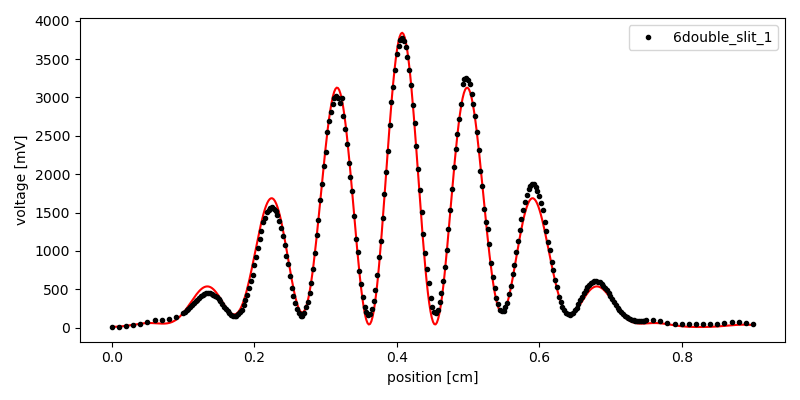
\includegraphics[width=7cm]{../results/laser(6_double_slit)_modified_fig.png}
        \caption{}
    \end{subfigure}
    \hfill
    \begin{subfigure}[b]{7cm}
      \centering
      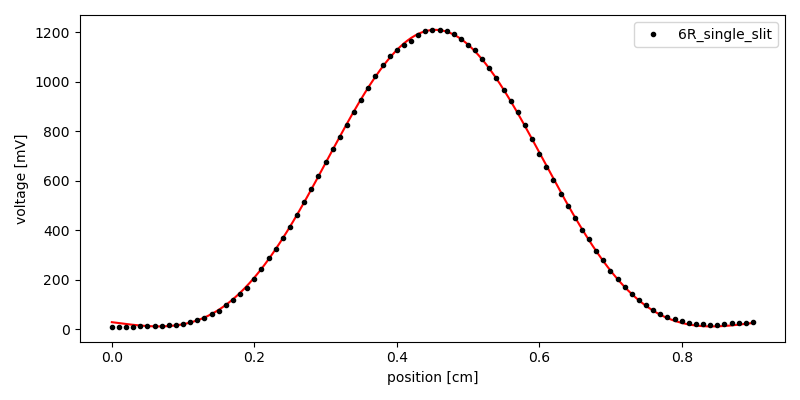
\includegraphics[width=7cm]{../results/laser(6_R_single_slit)_modified_fig.png}
      \caption{}
  \end{subfigure}
  \hfill
  \centering
  \begin{subfigure}[b]{7cm}
    \centering
    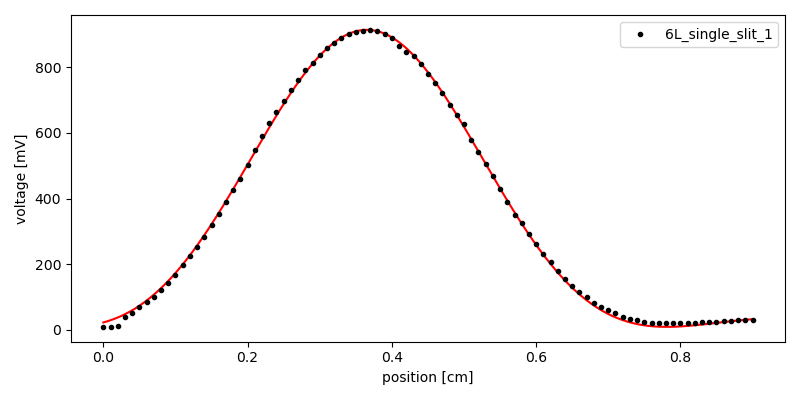
\includegraphics[width=7cm]{../results/laser(6_L_single_slit)_modified_fig.png}
    \caption{}
  \end{subfigure}
  \hfill
    \caption{Detected voltage [mV] - position [cm] plot of Slit No. 14, (a) double slit, (b) right side single slit, (c) left side single slit in the black dot.
        The red line is LBF fit results.
     }
    \label{fig: 14_laser_plot}
  \end{figure}

\begin{figure}[H]
    \begin{tabular}{  m{0.6cm}|m{2cm}|m{1.7cm}|m{2cm}|m{2.3cm}|m{2.3cm}|m{1cm} } 
        exp & c [mm]& I[mV] & $d_1$ [cm] & $d_2$ [mm] & $\Gamma$ & $R^2$ \\ \hline \hline
        all& $4.075 \pm 0.001$& $4100 \pm 328$& $1.309 \pm 0.01$& $0.9339 \pm 0.003$& $0.5433 \pm 0.001$& 0.9928\\ \hline 
        R& $ 4.541 \pm 0.001$& $1294 \pm 2$& $ 1.194 \pm 0.01$& & $ 0.0949 \pm 0.002$& 0.9999\\ \hline 
        L& $ 3.652 \pm 0.001$& $977.0 \pm 5.3$& $1.276 \pm 0.01$&& $ 0.101 \pm 0.06$& 0.9994\\ \hline 
    \end{tabular}
    \caption{Parameter statics of \ref{fig: 14_laser_plot}, experiment results of Slit No. 14.}
    \label{fig: 14_laser_parmeters}
\end{figure}

The pair results of Silt No. 15 are illustrated in Fig. \ref{fig: 15_laser_plot}, \ref{fig: 15_laser_parmeters}.
The data is also verified by the statistical criteria except for the $\Gamma$ value. 
The pair results of Silt No. 16 are illustrated in Fig. \ref{fig: 16_laser_plot}, \ref{fig: 16_laser_parmeters}.
The data is also verified by the statistical criteria except for the $\Gamma$ value. 

\begin{figure}[H]
    \begin{subfigure}[b]{7cm}
        \centering
        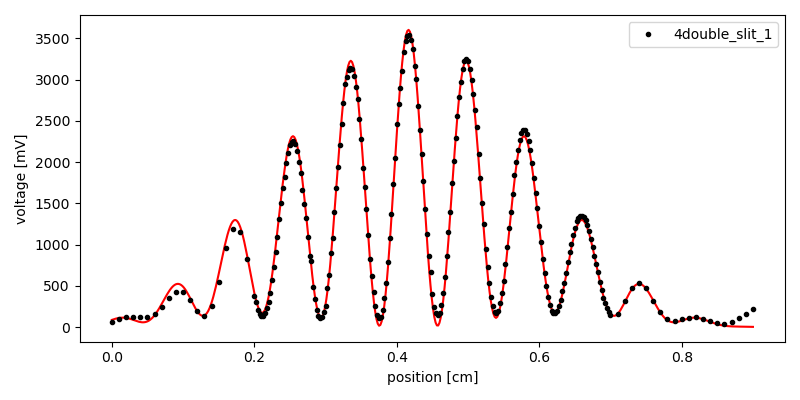
\includegraphics[width=7cm]{../results/laser(4_double_slit)_modified_fig.png}
        \caption{}
    \end{subfigure}
    \hfill
    \begin{subfigure}[b]{7cm}
      \centering
      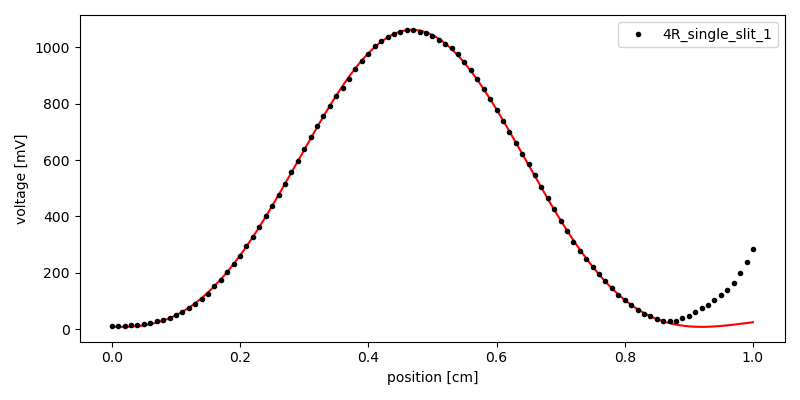
\includegraphics[width=7cm]{../results/laser(4_R_single_slit)_modified_fig.png}
      \caption{}
  \end{subfigure}
  \hfill
  \centering
  \begin{subfigure}[b]{7cm}
    \centering
    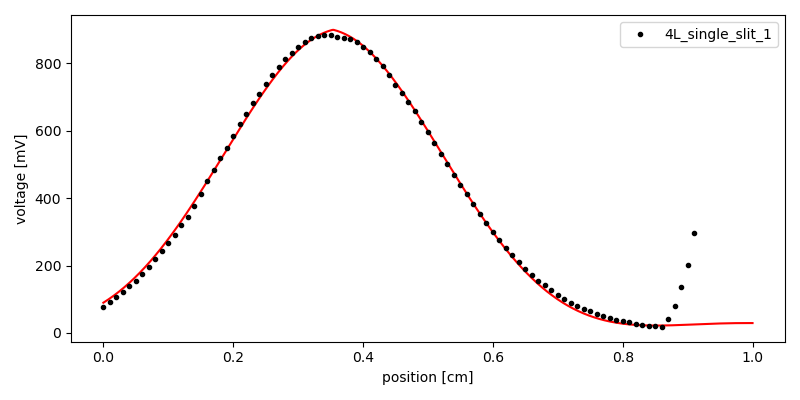
\includegraphics[width=7cm]{../results/laser(4_L_single_slit)_modified_fig.png}
    \caption{}
  \end{subfigure}
  \hfill
    \caption{Detected voltage [mV] - position [cm] plot of Slit No. 15, (a) double slit, (b) right side single slit, (c) left side single slit in the black dot.
        The red line is LBF fit results.
     }
    \label{fig: 15_laser_plot}
  \end{figure}

\begin{figure}[H]
    \begin{tabular}{  m{0.6cm}|m{2cm}|m{1.7cm}|m{2cm}|m{2.3cm}|m{2.3cm}|m{1cm} } 
        exp & c [mm]& I[mV] & $d_1$ [cm] & $d_2$ [mm] & $\Gamma$ & $R^2$ \\ \hline \hline
        all& $4.164 \pm 0.001$& $3852 \pm 160$& $1.544 \pm 0.01$& $0.8202 \pm 0.003$& $0.03604 \pm 0.001$& 0.9961\\ \hline 
        R& $4.683 \pm 0.001$& $1134 \pm 1$& $1.393 \pm 0.01$& &$0.088 \pm 0.001$& 0.9999\\ \hline 
        L& $3.539 \pm 0.001$& $961.4 \pm 16.6$& $1.426 \pm 0.01$& &$0.2208 \pm 0.001$& 0.9988\\ \hline 
    \end{tabular}
    \caption{Parameter statics of \ref{fig: 15_laser_plot}, experiment results of Slit No. 15.}
    \label{fig: 15_laser_parmeters}
\end{figure}

\begin{figure}[H]
  \begin{subfigure}[b]{6cm}
      \centering
      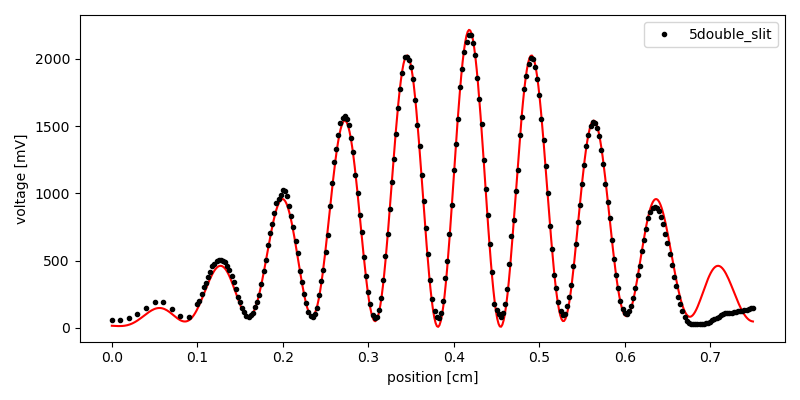
\includegraphics[width=6cm]{../results/laser(5_double_slit)_modified_fig.png}
      \caption{}
  \end{subfigure}
  \hfill
  \begin{subfigure}[b]{6cm}
    \centering
    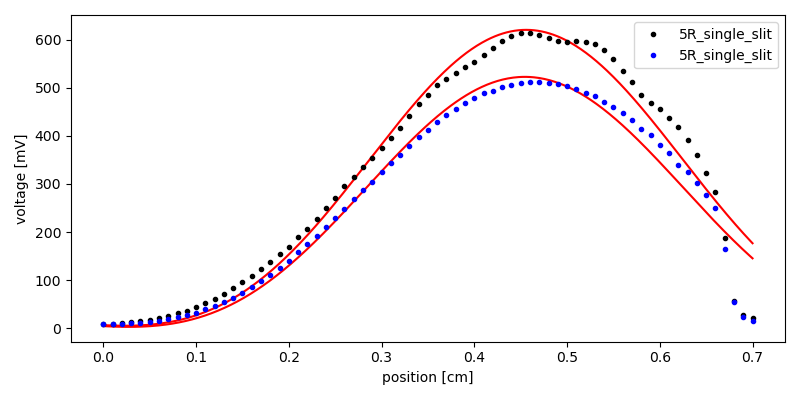
\includegraphics[width=6cm]{../results/laser(5_R_single_slit)_modified_fig.png}
    \caption{}
\end{subfigure}
\hfill
\centering
\begin{subfigure}[b]{6cm}
  \centering
  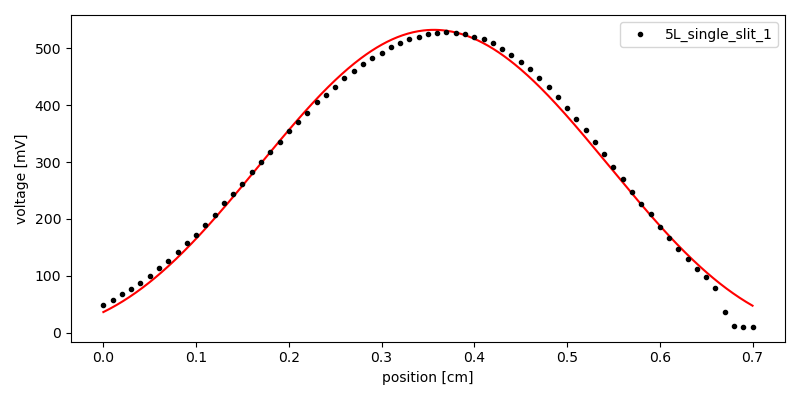
\includegraphics[width=6cm]{../results/laser(5_L_single_slit)_modified_fig.png}
  \caption{}
\end{subfigure}
\hfill
  \caption{Detected voltage [mV] - position [cm] plot of Slit No. 16, (a) double slit, (b) right side single slit(two trial is both plotted), (c) left side single slit in the black dot.
      The red line is LBF fit results.
   }
  \label{fig: 16_laser_plot}
\end{figure}

\begin{figure}[H]
  \begin{tabular}{  m{0.6cm}|m{2cm}|m{1.7cm}|m{2cm}|m{2.3cm}|m{2.3cm}|m{1cm} } 
      exp & c [mm]& I[mV] & $d_1$ [cm] & $d_2$ [mm] & $\Gamma$ & $R^2$ \\ \hline \hline
      all& $4.182 \pm 0.001$& $2370 \pm 111$& $1.505 \pm 0.01$& $0.735 \pm 0.003$& $0.02939 \pm 0.001$& 0.9923\\ \hline 
      R1& $4.560 \pm 0.001$& $662.8 \pm 139$& $1.33 \pm 0.01$& &$0.0953 \pm 0.0058$& 0.9655\\ \hline 
      R2& $4.545 \pm 0.001$& $558.4 \pm 80.6$& $1.326 \pm 0.01$& &$0.0727 \pm 0.0070$& 0.9695\\ \hline 
      L& $3.565 \pm 0.001$& $569.4 \pm 12.2$& $1.436 \pm 0.01$& &$0 \pm 0.000748$& 0.9926\\ \hline 

  \end{tabular}
  \caption{Parameter statics of \ref{fig: 16_laser_plot}, experiment results of Slit No. 16.}
  \label{fig: 16_laser_parmeters}
\end{figure}

The errors of $d_i$ are usually cut in order of measurement error, the fitting covariances are too small to be disregarded.
The system has the ambiguity of one external parameter, I believe the wavelength of the light source is $620 [nm]$ to establish $\sigma, \Delta$.
Fig. \ref{fig: laser_slit_spec} is the table of measured results of each slit number.
$\sigma_{R,L}$ are single slit width of each side, and $\sigma$ is fitted slit width parameter in double slit.
It is definite that $\sigma$ values are the same in the range of error, the criteria and assumption hold.

\begin{figure}[H]
  \centering
  \begin{tabular}{  m{2cm}|m{2.5cm}|m{2.5cm}|m{2.5cm}|m{2.5cm}} 
    Slit No. & $\sigma_R [mm]$ &$\sigma_L [mm]$ &$\sigma [mm]$ & $\Delta [mm]$ \\ \hline \hline
    14 &   $0.0279 \pm 0.001 $& $ 0.0261 \pm 0.001 $ & $0.0255  \pm 0.001 $  & $0.357  \pm 0.0003 $ \\ \hline
    15 &  $0.0240  \pm 0.001 $ & $0.0234 \pm 0.001 $ & $0.0216   \pm 0.001 $ & $0.407  \pm 0.0003 $\\ \hline
    16 &  $0.251  \pm 0.001 $ & $0.0232 \pm 0.001 $ & $0.0222 \pm 0.001 $   & $ 0.454  \pm 0.0002 $   \\ 
    
  \end{tabular}
  \caption{The slit width $\sigma_R, \sigma_L, \sigma$ and distance between two slit $\Delta$ of each Slit number}
  \label{fig: laser_slit_spec}
\end{figure}

Finally, the $\Gamma$ value is too widely distributed in various experiment settings.
Theoretically, the $\Gamma$ has the physical meaning of wavelength dispersion of the laser, which must have the same value nonrelated to the settings.
However, the mean square error value is too sensible to the differ of $\Gamma$, each fitting results are untrustable.
In each, the true values of $\Gamma_0$, $Err(I, I(;\Gamma))$ are the global minimum by its definition, but the optimizer will fall in the local minima of $\Gamma$.
But the local minima are located in 6D parameter space junked with other parameters $c, d_i, I$.
Therefore, I make a clever idea to break through this problem.
Let $Err(I_1(exp), I_2(parameters))$ denote the error of the measurement and fitting function.
$I_1$ is the experimental results of $(x, I)$ pairs in the experiment setting, I write $(exp)$ as respective indices of the whole experiment setting, such as (Slit No. 14, Align trial 5, double slit experiment) is one of the experiment setting indices.
$I_2$ is a function $I(x,param)$.
Then the $Err(I_1, I_2)$ is defined as equation \ref{equation: error_function} to exclude the effect of numbers in each experiment type.
$M(I)$ is the mean value of the set.

\begin{align}
  &s_{res} = \sum_{(x,I)} (I_1(x)-I_2(x,param))^2 \nonumber\\
  &s_{tot} = \sum_{(x,I)}(I- M(I))^2 \nonumber\\
  &Err(I_1, I_2) = \frac{s_{res}}{ s_{tot}} = 1-R^2 \label{equation: error_function}
\end{align}

Then the total error function $Err(\Gamma)$ is defined as equation \ref{equation: error_function_Gamma}.
For fixed $\Gamma$, fit parameters to every experiment the sum of minimized error is the error function of $\Gamma$.

\begin{equation}
  Err(\Gamma) = \sum_{(exp)} \min_{(param)} Err(I_1 (exp), I_2(param, \Gamma))
  \label{equation: error_function_Gamma}
\end{equation}

Fig. \ref{fig: laser_dispersion} is the plot of $Err(\Gamma)$.
The global minimum is easily found by $0.043$, which means the wavelength FWHM value $\gamma = \Gamma \times \lambda = 28.8 [nm]$.
The published FWHM is $\gamma = 20 [nm]$, which means this fitting is right.
The standard error of this value is not affordable, since this fitting consumes a lot of computing complexity, last 20 minutes, the covariances are hard to calculate.

\begin{figure}[H]
  \centering
  \begin{subfigure}[b]{7cm}
      \centering
      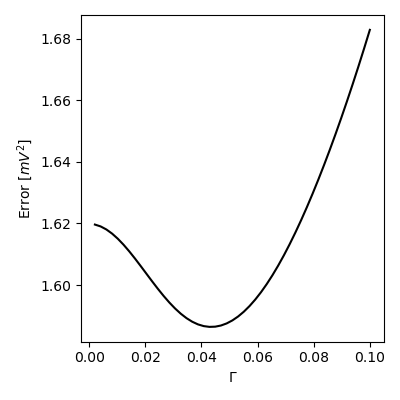
\includegraphics[width=7cm]{../results/laser_wavelength_dispersion.png}
      \caption{}
  \end{subfigure}
  \hfill
  \caption{Error [$mV^2$] - $\Gamma$ results of the measured data. it reaches the global minimum at $0.043$.}
  \label{fig: laser_dispersion}
\end{figure}

\subsection{PMT Threshold}
 The lower boundary and upper boundary of HV are required in the preset of the single photon limit experiment.
 In the dark, the unwanted PCIT occurs following equation \ref{equation: PMT}.
 The fitting result is sufficiently accurate in the dark condition.
 But, in the enlighten condition the fitting quite does not work well.
 The saturation of the amplifier might be the first reason, or the PCIT counting issue may occur cause of the fact that the time interval between peaks is too short to count.

 \begin{figure}[H]
  \centering
  \begin{subfigure}[b]{7cm}
      \centering
      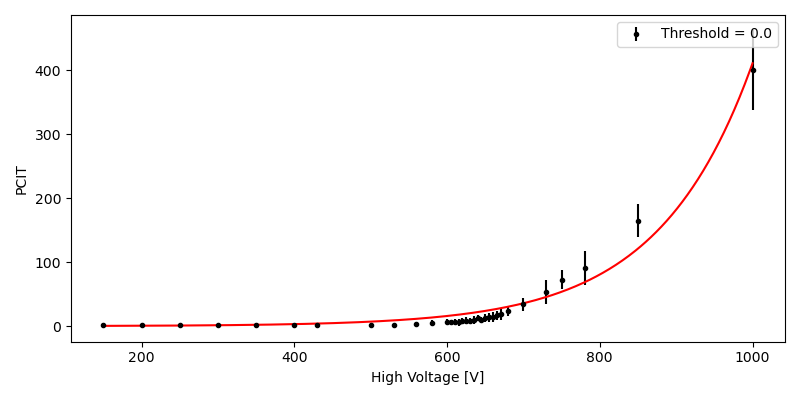
\includegraphics[width=7cm]{../results/PMT_upper_boundary_(0.0).png}
      \caption{}
  \end{subfigure}
  \hfill
  \begin{subfigure}[b]{7cm}
    \centering
    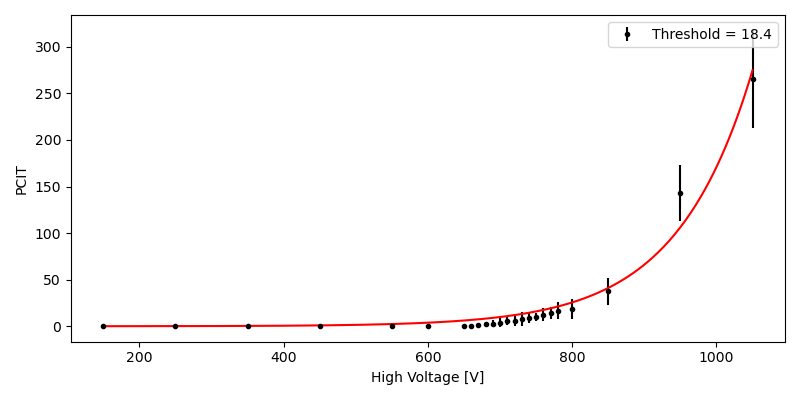
\includegraphics[width=7cm]{../results/PMT_upper_boundary_(18.4).png}
    \caption{}
\end{subfigure}
\hfill
  \caption{PCIT - HV [V] plots in threshold voltage (a) 0.00, (b) 18.4 [mV] in black dots,
    the red line is the fitting of $N(V) = a e^{bV}$
  }
  \label{fig: PMT_upper_boundary}
\end{figure}
\begin{figure}[H]
  \centering
  \begin{tabular}{  m{4cm}|m{2.5cm}|m{2.5cm}|m{2.5cm}} 
    Threshold [mV]& a& b$[V^{-1}$]& $R^2$ \\ \hline \hline
    0.0& $0.12 \pm 0.01$& $0.0081 \pm 0.001$& 0.9716\\ \hline 
    18.4& $0.012 \pm 0.01$& $0.0095 \pm 0.001$& 0.9756\\
  \end{tabular}
  \caption{The parameter of Fig. \ref{fig: PMT_upper_boundary}}
  \label{fig: PMT_upper_boundary_statics}
\end{figure}

Fig. \ref{fig: PMT_boundary} is the PCIT - HV plots in different bulb intensities.
Fig. \ref{fig: PMT_boundary}(b), the data of bulb intensity 1,2 is too small to distinguish from dark signal even in high HV values.
Therefore, I used only 3,4,5 intensities of bulb light and a threshold of 18.4 [mV].
Also, I chose the HV value where the $d(\Delta N)/dV = 0$, the highest resolution region, $HV = 720 [V]$
The threshold is accurate at $18.4 [mV]$, double-checked with an oscilloscope.
In HV $674 [V]$, PCIT value is $450 \pm 20$, where threshold $18.4 [mV]$ oscilloscope count is $445 \pm 25$
at the threshold $17.6 [mV]$ and $19.2 [mV]$, the oscilloscope counts are $661 \pm 33$ and $290 \pm 13$ respectively.
Which determines the threshold voltage as $18.4 \pm 0.4 [mV]$.

\begin{figure}[H]
  \centering
  \begin{subfigure}[b]{10cm}
      \centering
      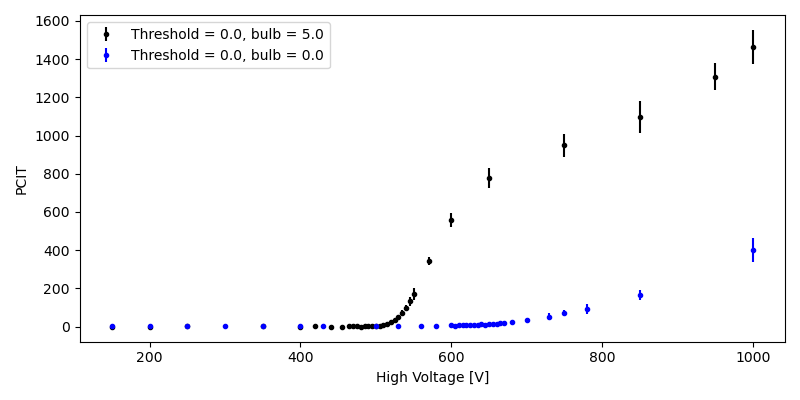
\includegraphics[width=10cm]{../results/PMT_boundary_(0.0).png}
      \caption{}
  \end{subfigure}
  \hfill
  \begin{subfigure}[b]{10cm}
    \centering
    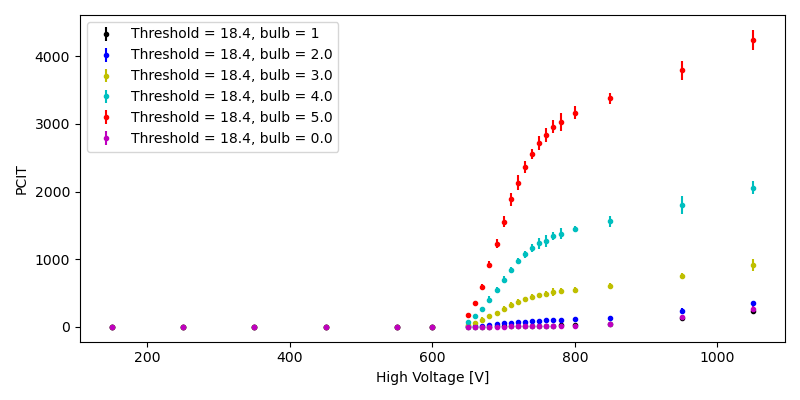
\includegraphics[width=10cm]{../results/PMT_boundary_(18.4).png}
    \caption{}
\end{subfigure}
\hfill
  \caption{PCIT - HV [V] plots in different bulb intensity and threshold (a) 0.00, (b) 18.4 [mV] in black dots.
  }
  \label{fig: PMT_boundary}
\end{figure}

For the rest of the experiment, the threshold and HV values are fixed at $18.4 [mV]$ and $720 [V]$.
The sensor slit alignment is done by measuring PCIT counts in plots of position, for different bulb intensities.
The zero signal offset average is $5.95 \pm 2.98$, all data are the subtracted results of the zero signal offset.
The Gaussian fitting does not give dramatic physical meaning, but the sensor slit center position is almost the $0.5 [cm]$, the evidence of successful alignment.
\begin{figure}[H]
  \centering
  \begin{subfigure}[b]{7cm}
      \centering
      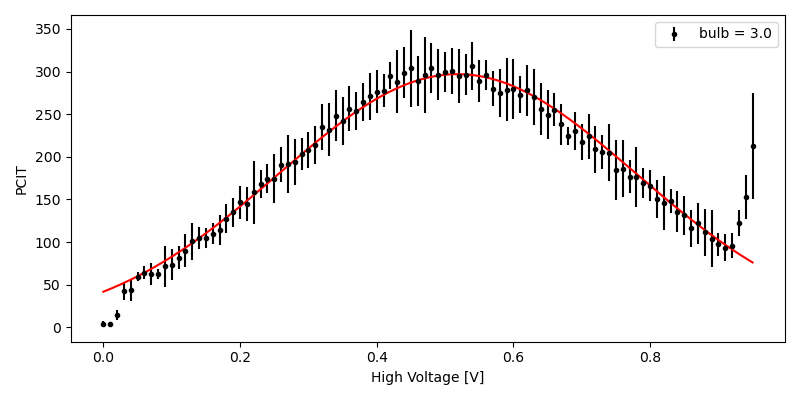
\includegraphics[width=7cm]{../results/sensor_slit_position_(3).png}
      \caption{}
  \end{subfigure}
  \hfill
  \begin{subfigure}[b]{7cm}
    \centering
    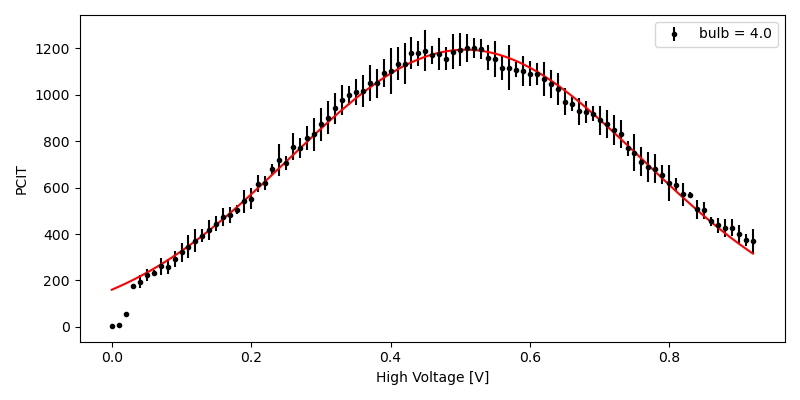
\includegraphics[width=7cm]{../results/sensor_slit_position_(4).png}
    \caption{}
\end{subfigure}
\centering
\hfill
\begin{subfigure}[b]{7cm}
  \centering
  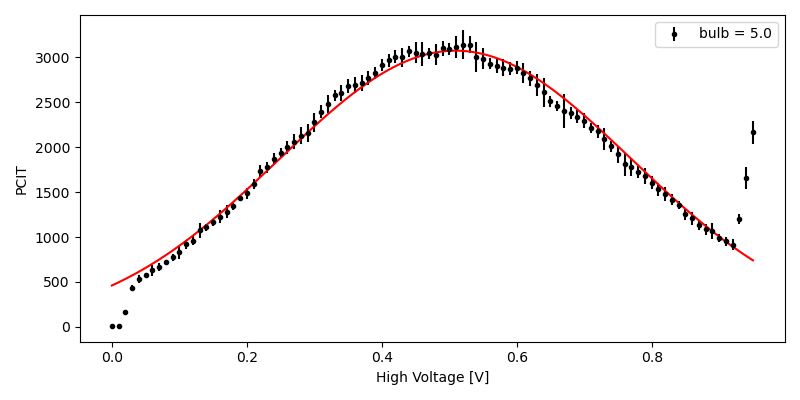
\includegraphics[width=7cm]{../results/sensor_slit_position_(5).png}
  \caption{}
\end{subfigure}
\hfill
  \caption{PCIT - position [cm] plots in different bulb intensity, no double slit condition results of bulb intensity (a) 3, (b) 4 (c) 5  in black dots.
    The red line is Gaussian fitting, $N(x) = A e^{-(x-m)^2/2\sigma^2}$.
  }
  \label{fig: sensor_slit_position}
\end{figure}
\begin{figure}[H]
  \centering
  \begin{tabular}{  m{1cm}|m{2.5cm}|m{2.5cm}|m{2.5cm}| m{2.5cm}} 
    bulb& A& $m[cm]$& $\sigma[cm]$& $R^2$ \\ \hline 
    3.0& $297.0 \pm 13.1$& $0.5182 \pm 0.001$& $0.2617 \pm 0.002$& 0.9477\\ \hline 
    4.0& $1194.0 \pm 47.3$& $0.5072 \pm 0.001$& $0.2529 \pm 0.004$& 0.9886\\ \hline 
    5.0& $3074.0 \pm 1477$& $0.5091 \pm 0.001$& $0.2613 \pm 0.002$& 0.9445\\ \hline 
    
  \end{tabular}
  \caption{The parameter of Fig. \ref{fig: sensor_slit_position}}
  \label{fig: sensor_slit_position_statics}
\end{figure}

The numerical approximation of the photon number is very important in setting a regime.
I assume that the Dark signal in the same HV is the value of PCIT counts by one photon.
This put its root in the simple claim, Dark signal is the result of the single excitation in the first PMT cathode.
About 5.95 PCIT counts is a photon excitation.
Therefore, 350, 1200, and 3000 PCIT each in the center of the screen is 50, 200, and 500 photons for bulb intensity 3, 4, and 5 respectively.
The slit transfers the photon order of $10^{-3}$, the photon emitted by the bulb is $5 \times 10^{4} , 2 \times 10^5 , 5 \times 10^5$ per second each.

\subsection{Bulb Experiment: Single Photon Limit}
In this subsection, three slits results are plotted and fitted respectively.
For each slit, two figures are posted.
The first figure is the PCIT - detector position [cm] plots of nine different experiment types, the double slit, and the single slits of each side, in differ of bulb intensities 3,4, and 5.
At each position, the PCIT counts are seven times measured for 1s, and average and standard deviation are plotted.
The second figure is the table containing parameter statics of previous plots respectively.
The row exp is the experiment type, all means the double slit case, and the R, L means the single slit of the right, left side.
$c, I,d_1,d_2,\Gamma$ is the position of the center of the screen, and the center PCIT count, the proper distances, and the dispersion coefficient respectively which are defined as equation \ref{equation: modified double slit}.

The pair results of Silt No. 14 are illustrated in Fig. \ref{fig: 14_bulb_plot}, \ref{fig: 14_bulb_parmeters}.
This result is the hard evidence of my explanation in $\Gamma$ that the $\Gamma$ parameter does not vary the result a lot, the physical quantity takes a similar size with each other in $1 \sigma$.
$c, d_1$ values are almost the same and the $I$ value ratio between bulb intensity is also similar, $1:3:7$ in rough calculation.
These two statistical conditions verify the fitting is valid.

\begin{figure}[H]
    \begin{subfigure}[b]{7cm}
        \centering
        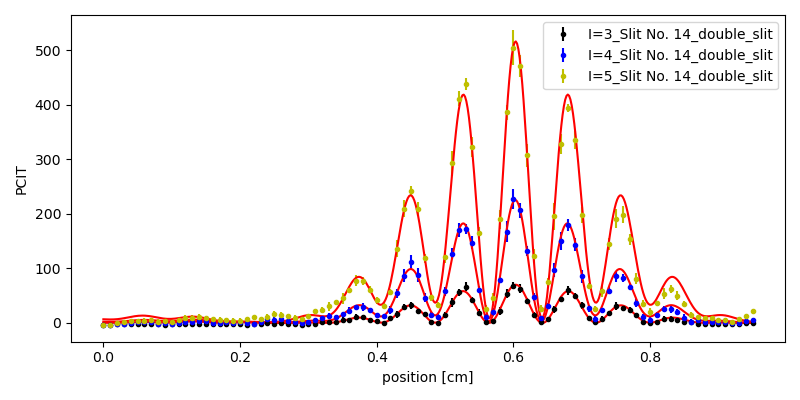
\includegraphics[width=7cm]{../results/bulb(14_double_slit)_fig.png}
        \caption{}
    \end{subfigure}
    \hfill
    \begin{subfigure}[b]{7cm}
      \centering
      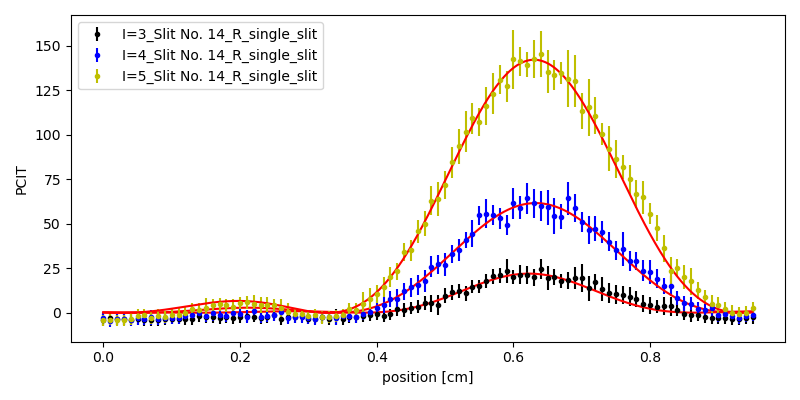
\includegraphics[width=7cm]{../results/bulb(14_R_single_slit)_fig.png}
      \caption{}
  \end{subfigure}
  \hfill
  \centering
  \begin{subfigure}[b]{7cm}
    \centering
    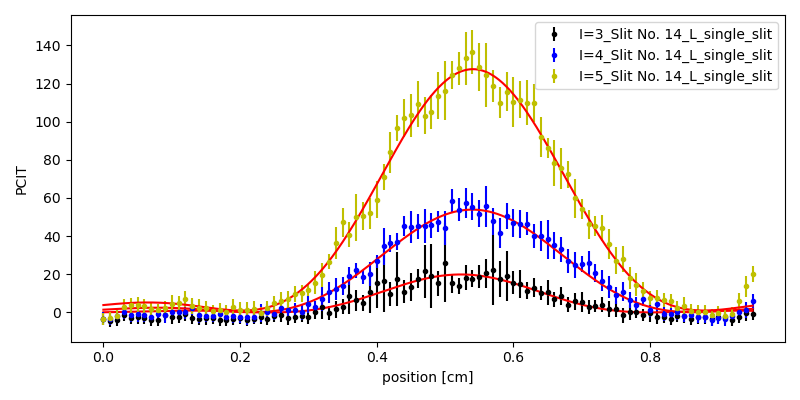
\includegraphics[width=7cm]{../results/bulb(14_L_single_slit)_fig.png}
    \caption{}
  \end{subfigure}
  \hfill
    \caption{PCIT counts - position [cm] plot of Slit No. 14, (a) double slit, (b) right side single slit, (c) left side single slit in the black dots, blue dots, and the yellow dots, bulb intensity of 3,4, and 5 each.
        The red line is LBF fit results.
     }
    \label{fig: 14_bulb_plot}
  \end{figure}

\begin{figure}[H]
    \begin{tabular}{  m{0.6cm}|m{0.3cm}|m{1.7cm}|m{1.7cm}|m{2cm}|m{2cm}|m{2cm}|m{1cm} } 
        exp & I & c [cm]& PCIT & $d_1$ [cm] & $d_2$ [cm] & $\Gamma$ & $R^2$ \\ \hline \hline
        \multirow{3}{*}{all}& 3 & $0.6034 $ & $75.00$& $1.063$& $0.07855$& $0.0207$& 0.9822\\ \cline{2-8}
                            & 4 & $0.6028$& $241.3$& $1.108$& $0.0779$& $0.0614$& 0.9943\\ \cline{2-8} 
                            & 5 & $0.6033$& $552.1$& $1.155$& $0.07815$& $0.0678 $& 0.9938\\ \hline 
        \multirow{3}{*}{R}  & 3 & $0.6227 $& $23.57$& $0.7574$&& $0.0674 $& 0.92\\ \cline{2-8}
                            & 4 &$0.6326$& $65.89$& $0.9232$&& $0.0000 $& 0.9809\\ \cline{2-8}
                            & 5 &$0.6303$& $151.9$& $0.9517$&& $0.0000$& 0.9972\\ \hline
        \multirow{3}{*}{L}  & 3 & $0.5231$& $21.26$& $0.8701$&& $0.0000$& 0.8779\\ \cline{2-8}
                            & 4 & $0.5398$& $57.6$& $1.014 $&& $0.0364 $& 0.98\\ \cline{2-8}
                            & 5 & $0.5408$& $136.3$& $1.045 $&& $0.0845$& 0.9914\\ \hline
    \end{tabular}
    \caption{Parameter statics of \ref{fig: 14_bulb_plot}, experiment results of Slit No. 14.
     The table is too small to write all of the standard errors.
     The errors of distance are $0.003$ [cm], and the $\Gamma$ value errors are too small in fitting covariance.
    }
    \label{fig: 14_bulb_parmeters}

\end{figure}


The pair results of Silt No. 15 are illustrated in Fig. \ref{fig: 15_bulb_plot}, \ref{fig: 15_bulb_parmeters}.
The pair results of Silt No. 15 are illustrated in Fig. \ref{fig: 16_bulb_plot}, \ref{fig: 16_bulb_parmeters}.
This result is the hard evidence of my explanation in $\Gamma$ that the $\Gamma$ parameter does not vary the result a lot, the physical quantity takes a similar size with each other in $1 \sigma$.
$c, d_1$ values are almost the same and the $I$ value ratio between bulb intensity is also similar, $1:3:7$ in rough calculation.
These two statistical conditions verify the fitting is valid.

\begin{figure}[H]
    \begin{subfigure}[b]{7cm}
        \centering
        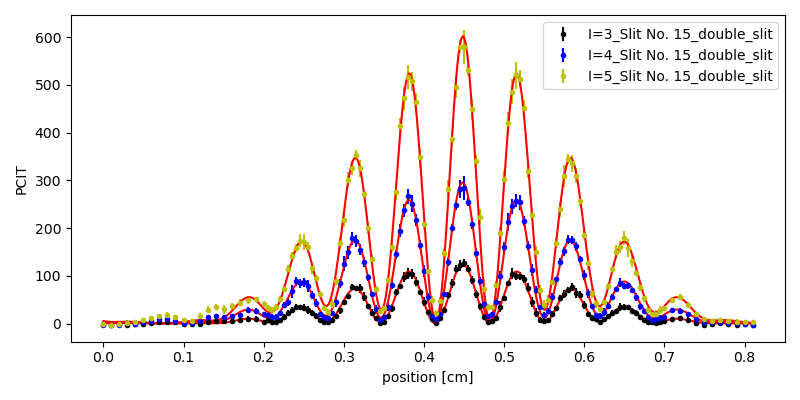
\includegraphics[width=7cm]{../results/bulb(15_double_slit)_fig.png}
        \caption{}
    \end{subfigure}
    \hfill
    \begin{subfigure}[b]{7cm}
      \centering
      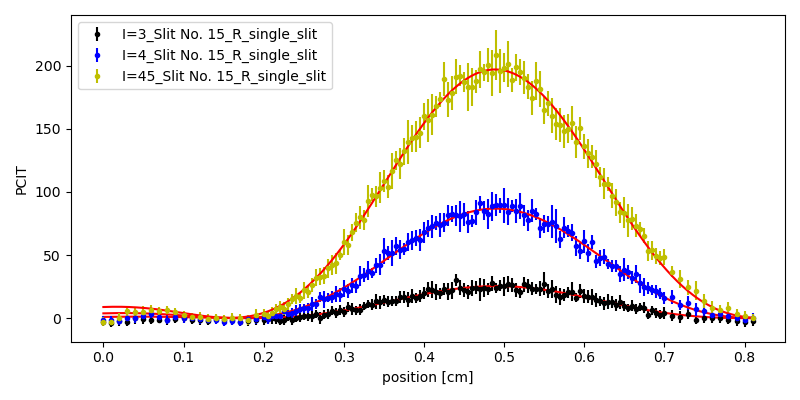
\includegraphics[width=7cm]{../results/bulb(15_R_single_slit)_fig.png}
      \caption{}
  \end{subfigure}
  \hfill
  \centering
  \begin{subfigure}[b]{7cm}
    \centering
    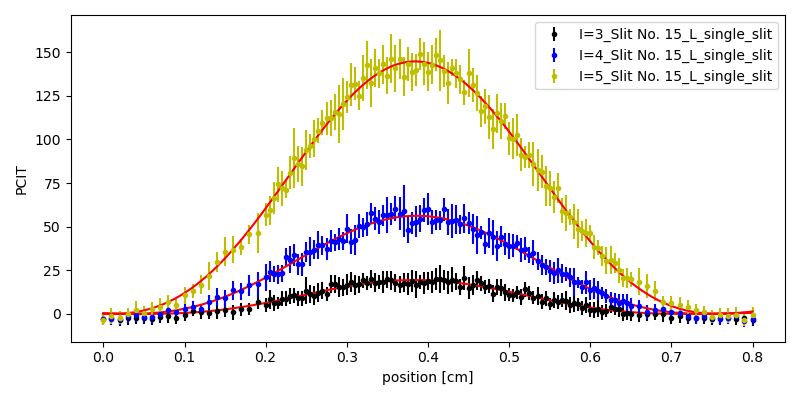
\includegraphics[width=7cm]{../results/bulb(15_L_single_slit)_fig.png}
    \caption{}
  \end{subfigure}
  \hfill
    \caption{PCIT counts - position [cm] plot of Slit No. 15, (a) double slit, (b) right side single slit, (c) left side single slit in the black dots, blue dots, and the yellow dots, bulb intensity of 3,4, and 5 each.
        The red line is LBF fit results.
     }
    \label{fig: 15_bulb_plot}
  \end{figure}

\begin{figure}[H]
    \begin{tabular}{  m{0.6cm}|m{0.3cm}|m{1.7cm}|m{1.7cm}|m{2cm}|m{2cm}|m{2cm}|m{1cm} } 
        exp & I & c [cm]& PCIT & $d_1$ [cm] & $d_2$ [cm] & $\Gamma$ & $R^2$ \\ \hline \hline
        \multirow{3}{*}{all}& 3 & $0.4484$& $132.4$& $1.139$& $0.06816$& $0.0287$& 0.9922\\ \cline{2-8}
                            & 4 & $0.4483$& $315.9$& $1.191$& $0.06801$& $0.0431$& 0.9951\\ \cline{2-8} 
                            & 5 & $0.4486$& $643.5$& $1.178$& $0.06798$& $0.0471$& 0.9946\\ \hline
        \multirow{3}{*}{R}  & 3 & $0.4908$& $27.15$& $0.9816$&& $0.0000$& 0.9613\\ \cline{2-8}
                            & 4 &$0.4891$& $92.77$& $1.018$&& $0.0215$& 0.9904\\ \cline{2-8}
                            & 5 &$0.4887$& $210.5$& $1.039$&& $0.0316$& 0.9955\\ \hline
        \multirow{3}{*}{L}  & 3 &  $0.3832$& $20.77$& $1.045$&& $0.0000$& 0.9559\\ \cline{2-8}
                            & 4 & $0.3862$& $60.12$& $1.120$&& $0.000125$& 0.9843\\ \cline{2-8}
                            & 5 & $0.3841$& $154.7$& $1.176$&& $0.000264 $& 0.9945\\ \hline
    \end{tabular}
    \caption{Parameter statics of \ref{fig: 15_bulb_plot}, experiment results of Slit No. 15.
     The table is too small to write all of the standard errors.
     The errors of distance are $0.003$ [cm], and the $\Gamma$ value errors are too small in fitting covariance.
    }
    \label{fig: 15_bulb_parmeters}
\end{figure}


\begin{figure}[H]
  \begin{subfigure}[b]{7cm}
      \centering
      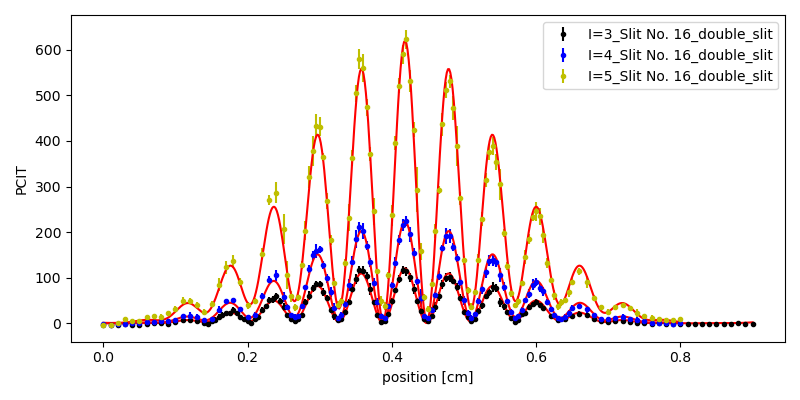
\includegraphics[width=7cm]{../results/bulb(16_double_slit)_fig.png}
      \caption{}
  \end{subfigure}
  \hfill
  \begin{subfigure}[b]{7cm}
    \centering
    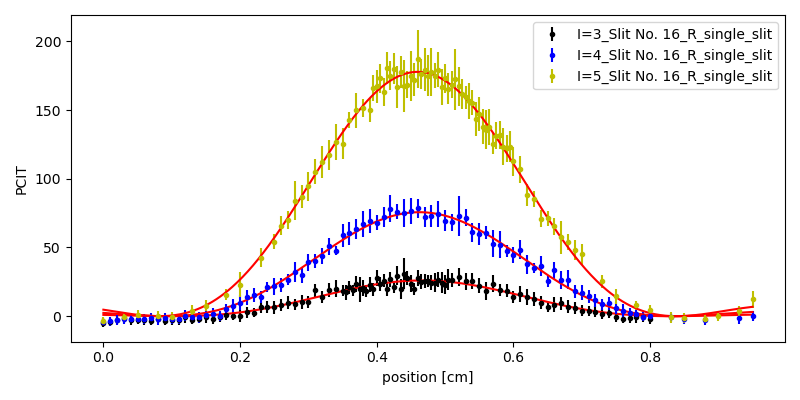
\includegraphics[width=7cm]{../results/bulb(16_R_single_slit)_fig.png}
    \caption{}
\end{subfigure}
\hfill
\centering
\begin{subfigure}[b]{7cm}
  \centering
  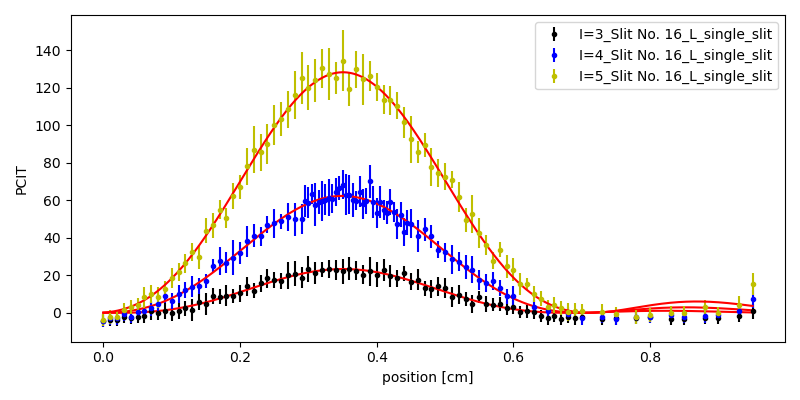
\includegraphics[width=7cm]{../results/bulb(16_L_single_slit)_fig.png}
  \caption{}
\end{subfigure}
\hfill
  \caption{PCIT counts - position [cm] plot of Slit No. 16, (a) double slit, (b) right side single slit, (c) left side single slit in the black dots, blue dots, and the yellow dots, bulb intensity of 3,4, and 5 each.
      The red line is LBF fit results.
   }
  \label{fig: 16_bulb_plot}
\end{figure}

\begin{figure}[H]
  \begin{tabular}{  m{0.6cm}|m{0.3cm}|m{1.7cm}|m{1.7cm}|m{2cm}|m{2cm}|m{2cm}|m{1cm} } 
      exp & I & c [cm]& PCIT & $d_1$ [cm] & $d_2$ [cm] & $\Gamma$ & $R^2$ \\ \hline \hline
      \multirow{3}{*}{all}& 3 & $0.4181$& $128.7$& $1.241 $& $0.0612 $& $0.0342$& 0.984\\ \cline{2-8}
                          & 4 & $0.4182$& $238.7$& $1.265$& $0.06125$& $0.0394$& 0.9896\\ \cline{2-8} 
                          & 5 &$0.4182$& $662.8 $& $1.282$& $0.06112  $& $0.0471$& 0.9898\\ \hline
      \multirow{3}{*}{R}  & 3 &$0.4663$& $27.77 $& $1.145 $&& $0.0000$& 0.9455\\  \cline{2-8}
                          & 4 &$0.4623$& $80.89$& $1.167$&& $0.0000$& 0.9889\\ \cline{2-8}
                          & 5 &$0.4600$& $190.0$& $1.191$&& $0.000285$& 0.9937\\ \hline
      \multirow{3}{*}{L}  & 3 & $0.3510$& $24.96$& $1.034$&& $0.0000$& 0.9651\\ \cline{2-8}
                          & 4 &$0.3496$& $66.62$& $1.105 $&& $0.0000$& 0.9856\\ \cline{2-8}
                          & 5 &$0.5408$& $136.3$& $1.045$&& $0.0846$& 0.9914\\ \hline
  \end{tabular}
  \caption{Parameter statics of \ref{fig: 16_bulb_plot}, experiment results of Slit No. 16.
   The table is too small to write all of the standard errors.
   The errors of distance are $0.003$ [cm], and the $\Gamma$ value errors are too small in fitting covariance.
  }
  \label{fig: 16_bulb_parmeters}
\end{figure}


The rest of the analysis of the results is the same as the laser experiment.
I trust the mid wavelength of the bulb filter,$\lambda_0 =  546 [nm]$,
The slit specs calculated by the bulb experiment are shown in Fig. \ref{fig: bulb_slit_spec}.
The $\Delta$ value of Slit No. 16, is $2 \sigma$ boundary but it is fine to have a total of one data out of $2 \sigma$ since it is possible to happen.
The error by $\Gamma$ function is displayed in Fig. \ref{fig: bulb_dispersion}, has its minimum value at $\Gamma =0.040$.
The wavelength dispersion $\gamma = \Gamma \lambda = 21.84 [nm]$, the FWHM value of the filter I can calculate.

\begin{figure}[H]
  \centering
  \begin{tabular}{  m{2cm}|m{2.5cm}|m{2.5cm}|m{2.5cm}|m{2.5cm}} 
    Slit No. & $\sigma_R [mm]$ &$\sigma_L [mm]$ &$\sigma [mm]$ & $\Delta [mm]$ \\ \hline \hline
    14 &   $0.027 \pm 0.003 $& $ 0.024 \pm 0.002 $ & $0.023  \pm 0.003 $  & $0.347  \pm 0.005 $ \\ \hline
    15 &  $0.026 \pm 0.002 $ & $0.025 \pm 0.001 $ & $0.023  \pm 0.002 $ & $0.399  \pm 0.0003 $\\ \hline
    16 &  $0.023 \pm 0.002 $ & $0.026 \pm 0.001 $ & $0.023   \pm 0.002 $ & $0.444  \pm 0.0003 $ \\ 
    
  \end{tabular}
  \caption{The slit width $\sigma_R, \sigma_L, \sigma$ and distance between two slit $\Delta$ of each Slit number}
  \label{fig: bulb_slit_spec}
\end{figure}


\begin{figure}[H]
  \centering
  \begin{subfigure}[b]{7cm}
      \centering
      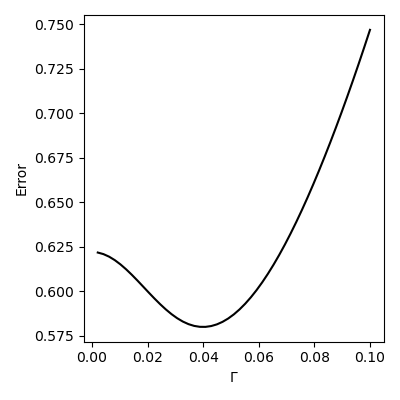
\includegraphics[width=7cm]{../results/bulb_wavelength_dispersion.png}
      \caption{}
  \end{subfigure}
  \hfill
  \caption{Error - $\Gamma$ results of the measured data. it reaches the global minimum at $0.040$.}
  \label{fig: bulb_dispersion}
\end{figure}

The dimensionless factor $\Gamma$ works with the wave packet length of the photon.
The wave packet length $\alpha$, has an order of Heisenberg criteria, $\alpha \Delta p \sim h$.
$\Delta p \sim \frac{h}{\lambda_0} \Gamma$, by definition of FWHM, can induce the order of $\alpha$.
$n$, the number of photons simultaneously transferring the slit, can be calculated as follows.

\begin{equation}
  n = \frac{ \frac{L}{c} \times j }{\frac{L}{\alpha}} = \frac{\alpha j}{c} \sim  \frac{\lambda_0 j}{c \Gamma}
\end{equation}

$j$ is the number of photons transferring the slit in unit time, $\frac{L}{c} \times j $ is the total number of photons transferring the slit in the u-channel.
The wave packet quantized the position to count, and the total length divided by packet size is the possible coherent position number, $\frac{L}{\alpha}$.
For the laser experiment, about $n = 30$ numbers of photons coherently pass through the slit, making the interference pattern.
For the bulb experiment, about $n = 4 \times 10^{-12}$ numbers of photon passes through the slit for the moment.
This means that the events of two or more coherent photons passing through the slit are impossible, or if it does, the statistical effect will hide the possibility at all.

\section{Summary}
I suggested the statistical criteria of fitting validity, to compare the same parameters in different condition experiments.
Also, I suggested dependent parameters $c, I,d_1, d_2$ and dimensionless parameter $\Gamma$ represents the dispersion ratio of the light.
Applying the criteria in the LBF model declares instability of parameter $\Gamma$, and makes a new method.
The method is to fit partially in total experiments, the plenty of data supports the reliability of its results.
It is trivial to prove that the partial fitting leads the total parameters to the global minimum.
The slit specification is 6 times verified in different experiments, the published value was right.
Interference pattern analysis in single photon limit is performed and proved that there are no mathematical changes with the multi-photon limit version experiment.
Doing all those jobs, for convenient code implementation is made.
I make the module helps to fit and plot at the same time, and to upgrade the package to calculate the dispersion ratio in the partial fitting method.



\bibliography{single_photon_interference_ref}
\bibliographystyle{plain}
\end{document}